\documentclass[10pt, a4paper]{report}

\usepackage[utf8]{inputenc}
\usepackage{polski}
\usepackage{a4wide}
\usepackage{fancyhdr}
\usepackage{lastpage}
\usepackage{tabularx}
\usepackage{graphicx}

\graphicspath{ {./images} }

%strona tytułowa
\begin{titlepage}

\title{\huge{\textbf{Sprawozdanie}}\\ gramatyk bezkontekstowych}
\author{Szymon Półtorak}
\date{}

\end{titlepage}

\renewcommand{\footrulewidth}{1pt}

\begin{document}
    \maketitle

    \renewcommand*\thesection{\arabic{section}} 
    
    \pagestyle{fancy}
    \fancyhf{}
    \rhead{Szymon Półtorak}
    \cfoot{Strona \thepage \hspace{1pt} z \pageref{LastPage}}
    
    \fancypagestyle{plain}{
        \rhead{Szymon Półtorak}
        \cfoot{Strona \thepage \hspace{1pt} z \pageref{LastPage}}
    }
    \tableofcontents
    \newpage

    \section{Treść Zadania}
    \begin{figure}[h]
        \begin{center}
            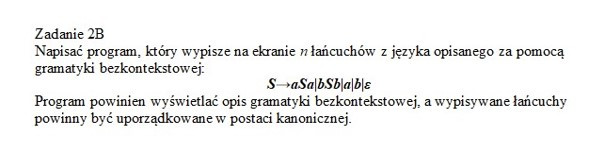
\includegraphics[scale=1]{photo1.jpg}
            \caption{Polecenie}
        \end{center}
    \end{figure}

    \section{Instrukcja obsługi programu}
    Żeby uruchomić program trzeba wejść w program Visual Studio 2019 Enterprise i po załadowaniu
    projektu trzeba wybrać opcję „Local Windows Debugger”.

    \begin{figure}[h]
        \begin{center}
            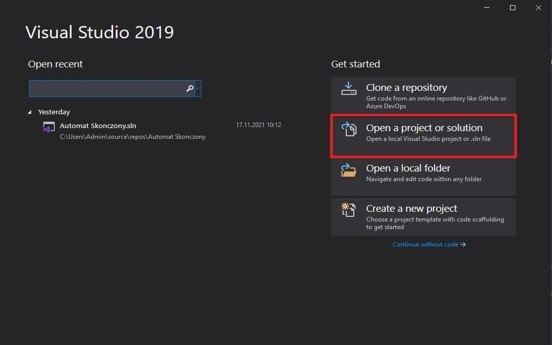
\includegraphics[scale=1]{photo2.jpg}
            \caption{Importowanie projektu}
        \end{center}
    \end{figure}
    \newpage

    \begin{figure}[h]
        \begin{center}
            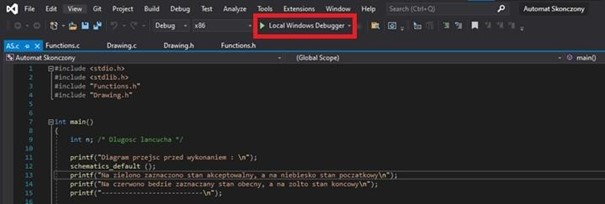
\includegraphics[scale=0.9]{photo3.jpg}
            \caption{Uruchamianie projektu}
        \end{center}
    \end{figure}

    Po uruchomieniu programu ukaże się nam okno, w którym będziemy mieli informację co robi
    program i jak opisana jest gramatyka. Program poprosi nas również o podanie, ile łańcuchów ma
    zostać wypisane. Po zatwierdzeniu klawiszem Enter program wypisze nam podaną przez nas liczbę
    łańcuch, które będą odpowiednio posortowane. Program zakończy działanie i poczeka aż użyjemy
    dowolnego klawisza do zamknięcia okna wiersza poleceń.

    \begin{figure}[h]
        \begin{center}
            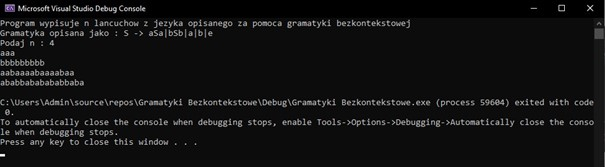
\includegraphics[scale=0.9]{photo4.jpg}
            \caption{Przykładowe wywołanie programu}
        \end{center}
    \end{figure}

    \section{Łańcuchy należące do danego języka}
    \begin{enumerate}
        \item bab,
        \item aaaaa,
        \item babab,
        \item abbabba,
        \item bababab,
        \item aaaaabaaaaa,
        \item abbabbabbabba,
        \item ababbbabababbbaba,
        \item baabbaababaabbaab,
        \item aabaaaaabbbaaaaabaa.
    \end{enumerate}

    \section{Bibliografia}
    \begin{enumerate}
        \item \textit{Język ANSI C}, Brian W. Kernighan, Dennis M. Ritchie,
        \item \textit{Wprowadzenie do teorii automatów, języków i obliczeń}, John Hopcroft, Jeffrey Ullman.
    \end{enumerate}

\end{document}